\section{Data Collection}
\label{S:D3}
In this study, an in-house developed tool, Virtual Immersive Reality Environment (VIRE)~\cite{farooq2018virtual}, is used to collect participants’ data while they were waiting on the sidewalk to cross an unsignalized intersection. The simulated unsignalized intersection is part of an existing congested street in Montreal, Canada. After an initial familiarization with VIRE, participants were asked to engage in three waiting conditions mentioned earlier. To capture the repetition concern, each task was conducted in 10 random simulation scenarios. Each trial would finish when the participant successfully crosses the street, with maximum allowable time of 60 seconds~\cite{sobhani2018impact}. Out of 42 participants, 17 were Females, the average age was 26, with 9 participants aged more than 30. Different variables were then generated based on participants collected data. As for the traffic simulation, car-following model and social force model were implemented for vehicular and pedestrian traffic, respectively. In \cref{fig:DVIRE}, VIRE set-up and a couple of participants in the experiment can be seen.
\begin{figure}
    \centering
    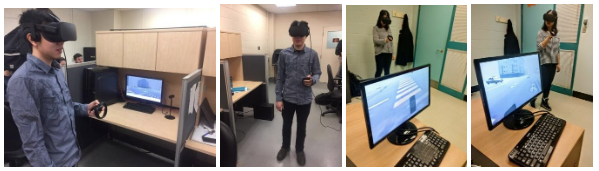
\includegraphics[scale=0.6]{chapter_3/figures/distract.png}
    \caption{VIRE setup and environment}
    \label{fig:DVIRE}
\end{figure}
